% !TeX root = ../main.tex
% -*- coding: utf-8 -*-

\chapter{绪论}
\label{chpt:introduction}
本章首先阐述本文的选题背景和意义,然后阐述论文的主要工作和创新点,最后介绍论文结构安排。

\section{研究背景与意义}
在软件生命周期中,随着外部环境的改变和用户需求的不断更新,必须不断修改软件系统以适应新的需求。这种改
变包括对软件缺陷的修复、新功能的添加和新技术的应用等。然而,随着软件系统的不断改变,代码结构变得越来
越复杂,导致软件质量的逐渐下降。在软件演化过程中,为了保证软件质量,提高用户体验,开发者有必要对软件
系统进行维护。

软件维护是指在软件发布后,为了修复缺陷、改善设计、提升性能等提高软件质量的目的而
进行的软件修改~\cite{IEEE1219}。在现代软件系统中,软件维护是贯穿软件生命周期的软
件活动,具有周期长、人员流动性强的特点。研究发现,在整个软件生命周期中,软件维护
和演化的成本占总成本的80\%以上~\cite{guimaraes1983managing, coleman1994using}。
由于软件维护占据整个生命周期的大部分,因此不能快速和可靠地维护软件往往带来巨大的
损失。

\subsection{软件维护的类型}

\begin{figure}
  \centering
  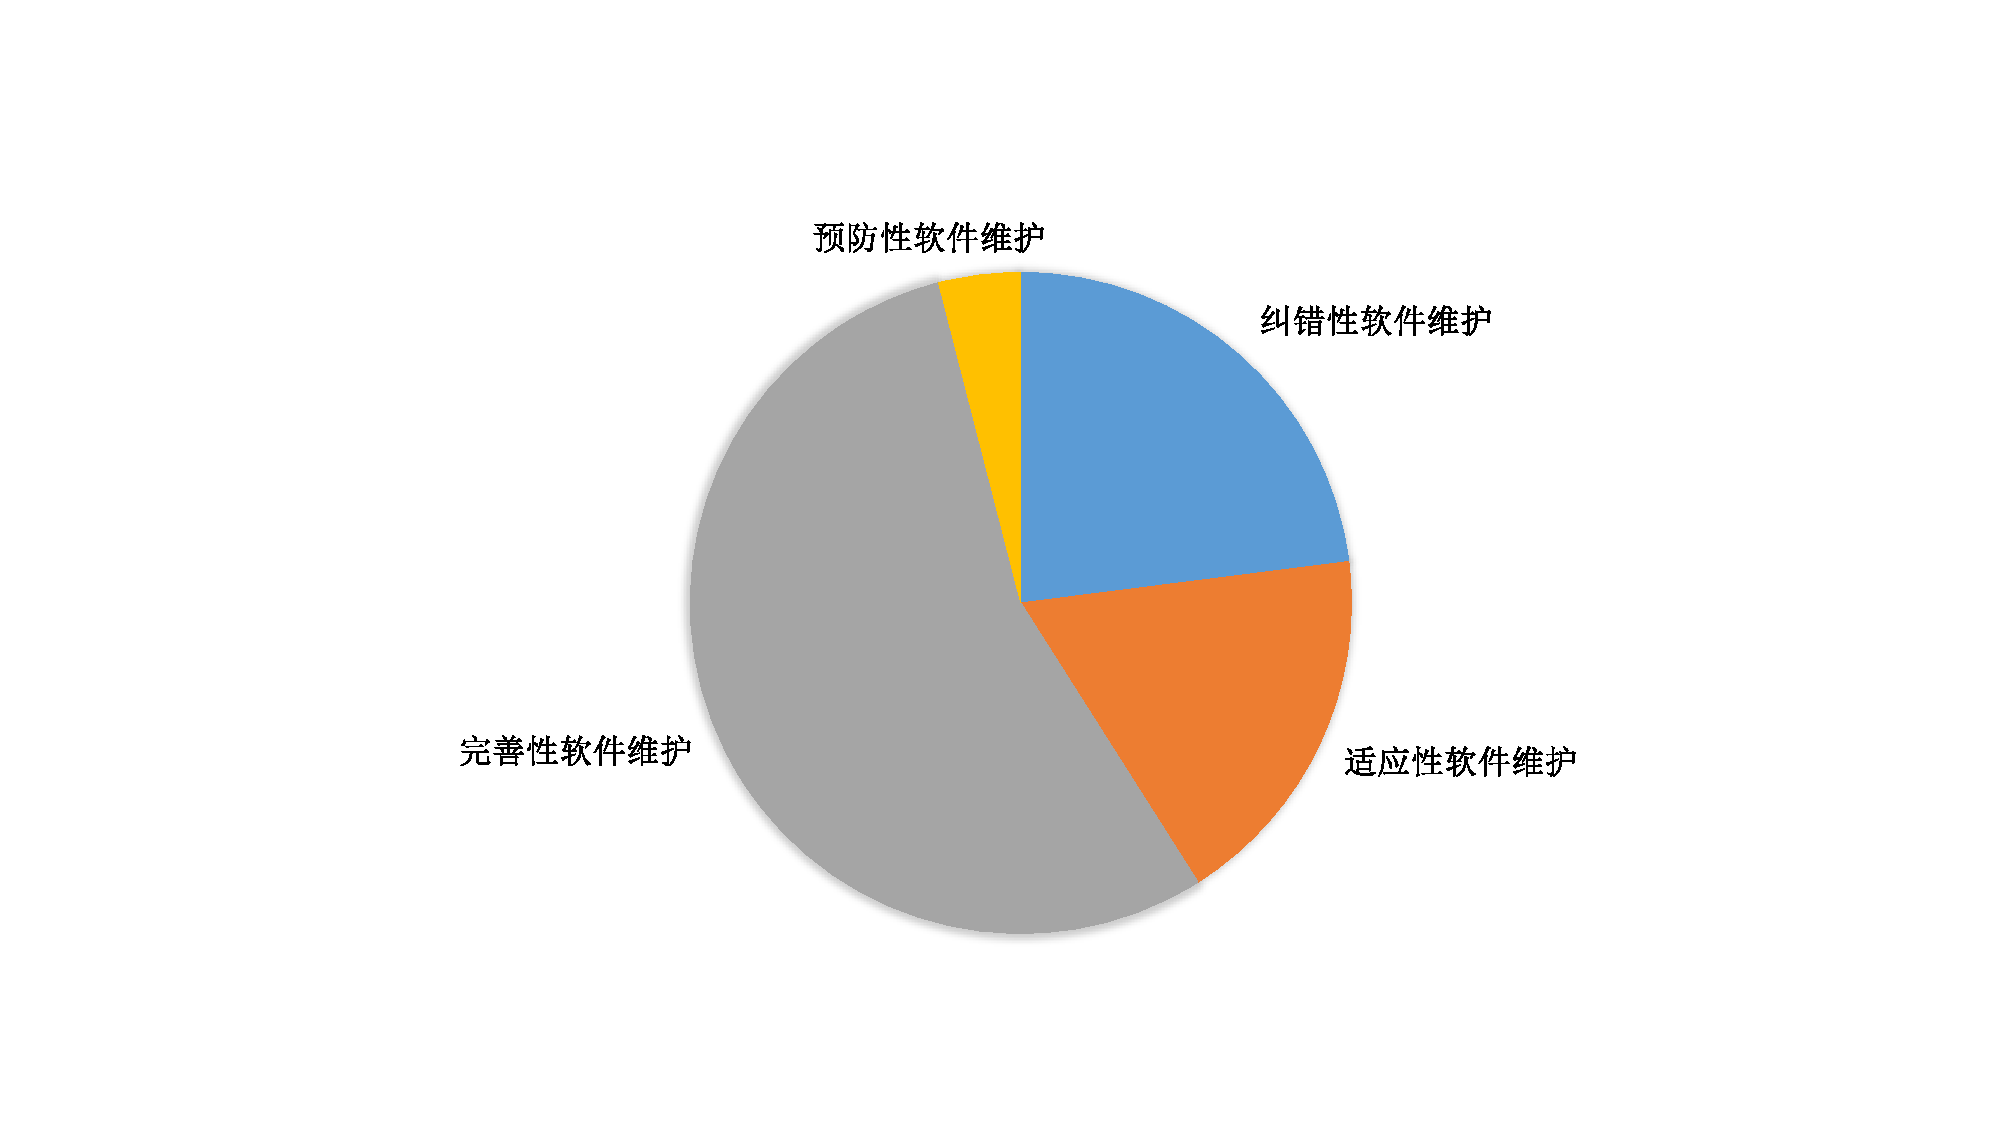
\includegraphics[width=0.6\linewidth]{maintenance.pdf}  
  \caption{\label{fig:maintenance}软件维护类型}
\end{figure}

软件维护主要包括四种类型,分别是纠错性软件维护、完善性软件维护、适应性软件维护和
预防性软件维护~\cite{lientz1978characteristics}。其中,纠错性软件维护指的是纠正
在开发过程中未被发现的、在实际应用中导致软件行为与预期不同的缺陷,是保障软件正确
性的重要手段;完善性软件维护指的是为了改进软件设计、提高软件运行效率和性能而对软
件系统做出的修改,是关系到软件系统质量的重要方面;适应性软件维护通常是为了让软件
系统能够适应技术和外部环境的变化而进行的软件维护;而预防性软件维护则是为了适应未
来外部环境和功能需求的改变,提前对软件系统做出的修改。从图~\ref{fig:maintenance}
中可以看出,在上述四种软件维护类型中,纠错性软件维护和完善性软件维护是最主要的两
种软件维护类型,共占软件维护总量约75\%。

随着科技的发展,软件系统已经深入到当代社会的各个方面。然而,由于软件开发过程中很
难发现所有潜在的缺陷,因此当软件系统投入使用时,可能会触发软件缺陷,导致系统不能
正常运行,从而给经济和社会带来巨大的损失。根据美国的标准与技术研究报告,软件缺陷
为美国带来每年高达600亿美元的损失,而及时发现软件缺陷则会为美国每年节约超220亿美
元~\cite{strate2013literature}。纠错性软件维护通过对软件缺陷的定位、诊断和修复,
能够及时发现并修改软件系统中存在的缺陷,是保障软件正确性的重要手段。

随着对软件系统的不断修改,软件系统渐渐偏离原来的设计,此时虽然保障了软件的正确
性,但软件的质量不断下降,导致软件维护的难度越来越高。在这种情况下,需要对软件进
行完善性维护,通过改善软件设计,提高软件系统的易读性、可维护性和可靠性等重要软件
质量因素,在延长软件系统寿命的同时降低软件维护成本。

研究发现,良好的软件质量能够有效减少缺陷的发生;同时,当软件系统存在缺陷时,易读
性和可维护性强的软件系统能够帮助维护人员尽早发现软件缺陷,从而提升纠错性软件维护
的效率~\cite{martin2009clean}。因此,在软件系统的迭代过程中,纠错性软件维护与完
善性软件维护通常是交替发生的。一方面,纠错性软件维护使软件能够正确运行,是完善性
软件维护的基础;另一方面,完善性软件维护通过降低软件维护难度、提升软件系统质量,
能够提高纠错性软件维护的效率,并减少新缺陷的引入。


\subsection{基于数据驱动的软件维护}
当代软件系统通常具备代码规模大、迭代周期短的特点,使得人工进行软件维护变得越来越
困难。一方面,软件维护所需要的时间和人力成本较高。软件维护通常建立在理解软件系统
的基础上,然而,随着软件规模的增大和代码复杂度的提高,软件系统的维护成本也随之越
来越高,即使是经验丰富的软件维护人员也很难快速掌握整个软件系统。另一方面,人工软
件维护的效果容易受到个体思维的影响,因此对软件维护人员的能力和经验要求较高。除此
以外,人员流动性也为人工进行软件维护带来了一定的困难。

自动化软件维护可以解决人工维护的效率低、易受个体思维影响的缺点,因此,很多研究者
致力于提出各种自动化、半自动化的技术来提高软件维护的效率和性能。例如,在纠错性软
件维护方面,研究者提出用自动化测试技术来代替传统的人工测试,从而解决人工测试中经
常发生的遗漏、思维惯性等问题,使测试更快、更可靠、更便宜。在完善性软件维护方面,
大多数集成开发环境,如Eclipse和IntelliJ IDEA等都提供了插件为软件重构提供技术支
持,而这样的插件是目前软件重构能够被广泛应用的重要原因之一
~\cite{griswold1993automated,tip2003refactoring,mens2005formalizing}。

虽然自动化软件维护能够提高维护效率、降低维护成本,但是由于软件维护的原因较为多
样、过程也较为复杂,目前很难制定一套完整而严密的规则来解决软件维护中的难题,因此
当前很多软件维护任务难以被完全自动化的技术所完成。例如,虽然自动化测试技术能够提
高软件测试的效率和性能,但是对于测试用例的执行结果仍然需要人工判定,自动预言测试
用例的预期行为仍是目前尚未解决的难题。同理,虽然大部分集成开发环境都已经支持软件
重构,但在软件重构的过程中仍然需要人工识别软件重构机会并决定如何进行重构,目前大
多数软件重构支持插件的作用仅仅是执行使用者指定的操作
~\cite{fowler1999refactoring, murphy2012we}。由于软件维护很难通过完全自动化实
现,因此在软件维护过程中仍然需要消耗维护人员大量的时间和精力。

数据挖掘为这种存在内部规律但很却难通过制定完美规则来解决的难题提供了一种新的解决
思路,即挖掘数据中的潜在规律作为问题的解决方案。目前成熟的开源社区和版本控制工具
(如CVS、Git、SVN等)已经为研究者们提供了大量的研究数据,包括软件系统的版本、规
模、复杂度和历史修改等。从数据的角度来理解软件系统,将软件维护问题转化为数据挖掘
问题,既能够有效避免对软件维护人员经验的依赖,又能够提高软件维护效率,减少软件维
护的时间和人力成本,因此成为了近几年软件工程领域的研究热点。目前机器学习和数据挖
掘算法已经被广泛应用于软件工程的很多领域,如缺陷预测
~\cite{menzies2007data,drown2009evolutionary,khoshgoftaar2010attribute}、代码生
成~\cite{maddison2014structured,ling2016latent}、缺陷定位
~\cite{malcov2013,nnfault2013}等。

本文主要针对纠错性和完善性软件维护中的关键难题,通过数据挖掘得到问题的解决方案,
提高软件维护的效率,从而更好地适应当代软件系统对于可靠性和快速迭代的需求。

\section{研究内容与创新点}
本文通过数据挖掘的方法对软件维护中最两种主要的软件维护类型进行研究,即纠错性和完
善性软件维护。其中,纠错性软件维护是保障软件正确性的重要手段,也是完善性软件维护
的基础;同时,完善性软件维护通过改善软件设计、提高软件的易读性和可维护性,能够有
效提升纠错性软件维护的效率,并减少软件缺陷的发生。

本文的研究内容与创新点主要包括:

(1)为了提高纠错性软件维护的效率,本文提出了基于相关统计量的缺陷定位方法。在软
件生命周期中,通常需要不断地对软件进行纠错性软件维护,使其越来越接近完全正确。本
文研究了基于覆盖分析的缺陷定位方法(Coverage-Based Fault Localization,CBFL),
其核心思想是被失效用例执行越多、成功用例执行越少的代码可疑度越高
~\cite{jones2005empirical},该方法由于计算成本较低而适用于大规模软件系统。由于现
有的基于覆盖分析的缺陷定位方法由于无法区分由不同缺陷引发的失效用例,导致缺陷之间
相互影响,从而影响多缺陷程序的定位效率。本文以测试用例作为样本,执行结果作为样本
的二分类标签,执行覆盖信息作为特征,将多缺陷定位问题转化为数据挖掘领域的特征选择
问题,选择有较大可能导致样本标签为``失效''的覆盖特征作为可疑代码。受Relief特征选
择算法启发~\cite{kira1992feature},本文提出了缺陷相关统计量,通过为每个测试用例
选择距离其最近的同类和异类测试用例,找到最有可能与失效用例由同一缺陷触发的另一个
失效用例,从而在一定程度上避免了不同缺陷之间的相互影响,提高了多缺陷定位的效率。

(2)为了提高完善性软件维护的效率,本文提出了基于梯度上升决策树的函数抽取重构机
会推荐模型。虽然纠错性软件维护能够提高软件的正确性,但随着对软件系统的不断修改,
软件质量越来越低,软件维护的难度也越来越高。为了提高软件质量,需要对软件系统进行
完善性软件维护,通过改进软件系统的设计结构,提高软件的易读性和可维护性。本文针对
最常见的软件重构类型之一,函数抽取(Extract Method)软件重构,提出了基于梯度上升
决策树的重构机会推荐模型。与传统的基于软件质量度量的重构机会推荐方法不同,本文通
过挖掘开源软件系统中的重构实例,学习函数抽取软件重构的内在规律,从而为软件维护人
员自动推荐函数抽取重构机会。在训练阶段,本文的特征提取算法在融合了复杂度、内聚度
和耦合度三个重要软件质量因素的同时,考虑了包括变量、类型、函数调用等多种程序元
素,通过构建关于函数抽取重构的概率模型,学习如何进行函数抽取重构;在推荐阶段,本
文为给定函数体生成所有合法的候选函数抽取重构机会,并使用训练好的模型为每个重构机
会分配一个概率,根据概率由高至低推荐给用户,从而提高完善性软件维护的效率。

(3)为了提高软件系统的易读性和可维护性,本文提出了基于层次注意力的函数名推荐模
型。在软件维护过程中,最耗费时间和精力的是阅读代码的过程~\cite{rugaber2000use}。
准确的函数名通过对函数的抽象概括,让软件维护人员不需要阅读代码细节,就可以理解函
数的大致功能,从而提高代码阅读的速度和软件维护的效率。本文通过挖掘GitHub上广受欢
迎的开源软件系统,学习函数命名的内在规律,从而为给定代码片段推荐合适的函数名。本
文提出了基于层次注意力的函数名推荐模型,该模型以编码-解码器模型
(Encoder-Decoder)为基本框架,将输入代码片段拆分为由多个代码基本块组成的序列,
每个代码基本块为一个词项序列;通过注意力机制分别学习词项对代码块、代码块对代码片
段的重要性,使模型能够识别对函数名预测有益的词项和代码基本块,最后通过集束搜索生
成具有概率的词项序列作为函数名推荐结果。

\section{论文结构安排}
\begin{figure}[htp]
  \centering
  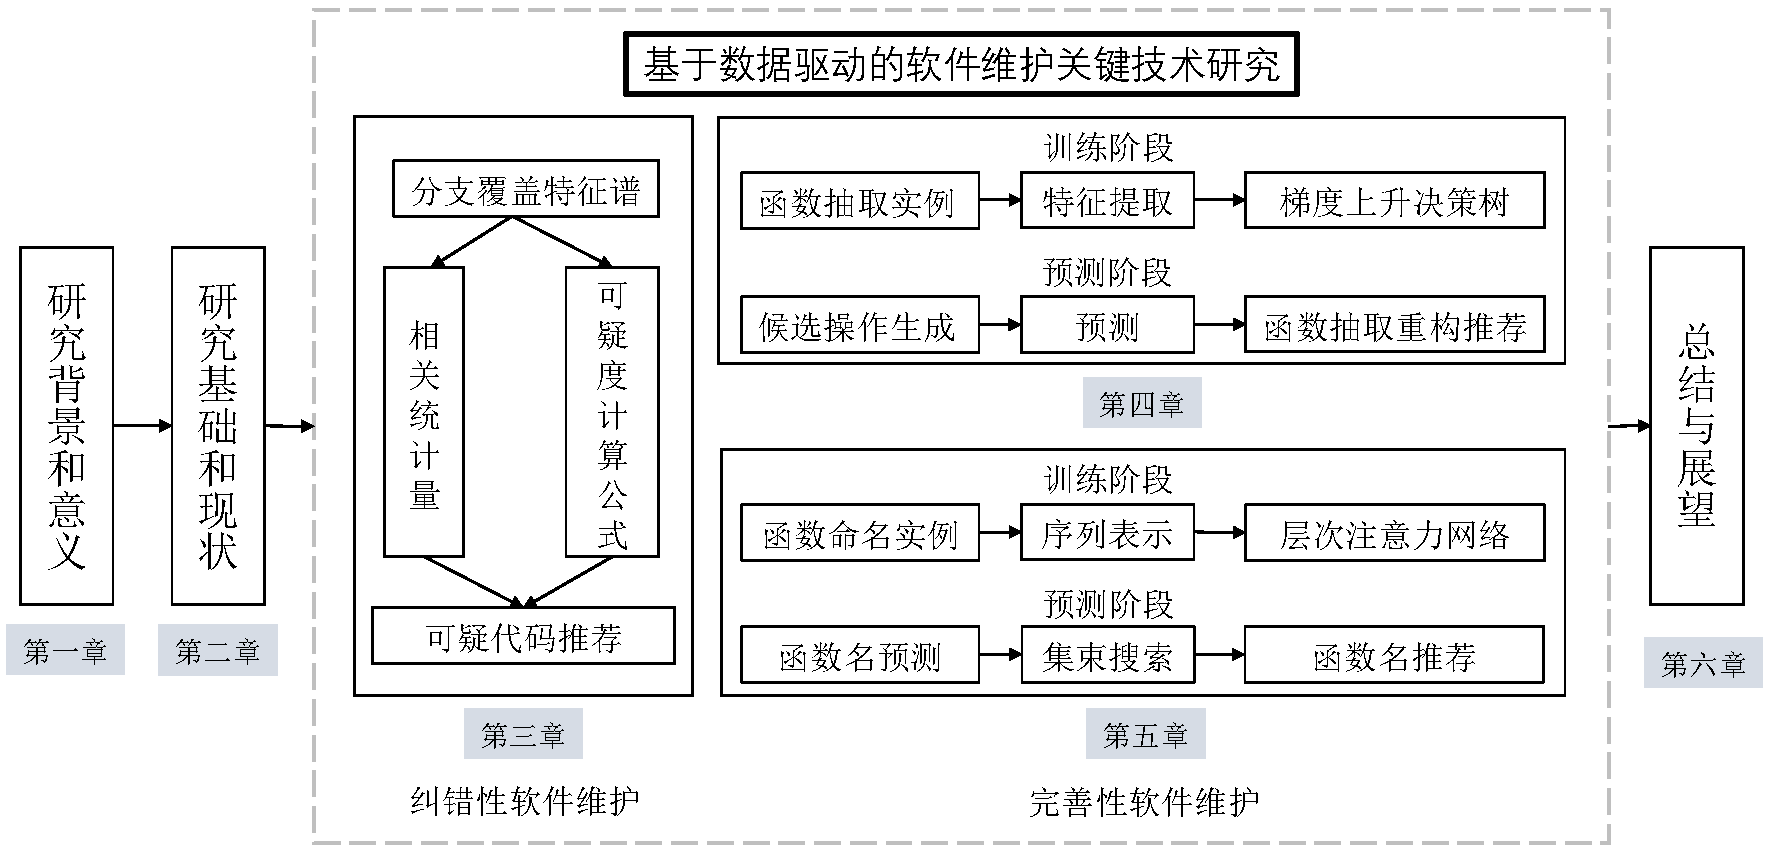
\includegraphics[width=1.0\linewidth]{org.pdf}
  \caption{论文组织结构}
  \label{fig:org}
\end{figure}

如图~\ref{fig:org}所示,本文共分为六章。首先,第一章介绍了本文研究的背景和意义,以及本文的主要研究内容和创新点。后续章节的内容如下:  

第二章介绍本文的研究基础与现状。本文的研究内容主要针对软件维护中最重要两个软件维
护类型,即纠错性维护和完善性维护。首先介绍了缺陷定位的相关研究工作;然后介绍了软
件重构的研究基础,包括软件质量和代码坏味的关系、软件重构类型和软件重构推荐方法的
研究基础和现状。

第三章提出了基于相关统计量的缺陷定位方法。首先介绍了基于覆盖分析的缺陷定位方法的
原理,然后描述了覆盖分析法在面对多缺陷程序时定位效率下降的问题,接着引入了特征选
择中的相关统计量概念,并提出了缺陷相关统计量来代替传统的可疑度计算公式,提升了多
缺陷程序的定位效率。最后在实验部分设计了关于单缺陷程序和多缺陷程序的两组对比实
验,通过与当前流行的基于覆盖分析的缺陷定位方法进行对比,评估了基于相关统计量的缺
陷定位方法的有效性。

第四章提出了基于梯度上升决策树的函数抽取重构机会推荐方法。首先介绍了方法的基本框
架,然后描述了特征提取算法,接着介绍了梯度上升决策树和函数抽取重构机会生成,最后
在实验部分通过与当前流行的函数抽取重构机会推荐工具进行对比实验,在两个训练数据集
和四个分类模型上证明了本章方法的有效性。

第五章提出了基于层次注意力的函数名推荐模型。首先介绍了编码-解码模型和基于层次注
意力模型的基本架构,然后分别对基于层次注意力的函数名推荐模型中的各个组成部分进行
描述,接着介绍了基于集束搜索的函数名推荐方法,最后在描述了本章的实验部分,通过在
10个开源软件系统上得对比实验,证明了基于层次注意力的函数名推荐模型的有效性。

第六章对本文进行总结,并展望接下来的研究方向。
